\documentclass[a4paper,10pt]{article}
\usepackage[utf8]{inputenc}
\usepackage[margin=0.7in]{geometry}     %% Margins
\usepackage{parskip}                    %% Tiny gaps after enter
\setlength\parindent{0pt}               %% Noindent for entire file
\usepackage[backend=biber, url=false]{biblatex}    %% Bibliography
\usepackage{graphicx}                   %% Allow image figures
\usepackage{subcaption}                 %% Allow image captions
\usepackage{hyperref}
\usepackage{cleveref}                   %% Smart figure references
\addbibresource{refs.bib}


%opening
\title{
  Model-Based Estimation of Functional Connectivity in Whole-Brain Multifiber Implant Calcium Dynamics in Behaving Mice\\
  %%
  \vspace{10pt}
  \small Report for 2019 Computational Psychiatry Course}
\author{Aleksejs Fomins}

\begin{document}

\maketitle

\section{Introduction}
Mesoscopic whole-brain imaging is a large field. A wide variety of measurement techniques, such as fMRI \cite{ogawa_brain_1990, belliveau_functional_1990, deyoe_functional_1994, buxton_modeling_2004, kiebel_dynamic_2008}, EEG \cite{wright_dynamics_1996, baillet_bayesian_1997, gross_dynamic_2001, kececi_quantitative_2008} and wide-field calcium imaging \cite{gilad_behavioral_2018, silasi_intact_2016, holtmaat_long_term_2009, dombeck_imaging_2007} are used to record functions of neuronal signals averaged over large neuronal populations. An important question is the capacity of recorded mesoscopic signals to explain observables external to the brain, such as sensory input, behaviour and learning, and vice versa.

An ideal latent variable model would be capable of accurately predicting the future values of mesoscopic activity and external observables based their past values. Given current state of the art data, the construction of a fully self-consistent mesoscopic model of a brain or its part is unlikely because, among others, such a model would struggle to account for a) heterogeneity of a neuronal population b) specificity of its response c) inputs from unobserved neuronal populations and external stimuli. However, it is not unreasonable to assume that brain activity can be decomposed into a spatio-temporal basis of increasing detail, allowing to have a progressively more accurate account of external observables.

An interesting latent variable of a network activity is the so-called Functional Connectivity \cite{friston_functional_2011, hutchison_dynamic_2013}. Loosely, it can be defined as the capacity of the value of one variable to be predictive of the value of another variable at a later time. FC is designed to indicate potential causal relationships between variables, however, far greater knowledge of the system is required to guarantee causality as the only possible explanation of FC \cite{wibral_directed_2014}. While it is frequently impossible to unambiguously estimate FC \cite{wibral_directed_2014}, standardized metrics of FC have been demonstrated to be predictive of working memory \cite{greicius_functional_2003, esposito_independent_2006}, daydreaming \cite{kucyi_dynamic_2014}, decision making \cite{lizier_multivariate_2010}, pathology \cite{sakoglu_classification_2009} and learning \cite{bassett_dynamic_2011}. Among others, the following model-free metrics for FC have been proposed: correlation \cite{greicius_persistent_2008, thompson_short_time_2012, viviani_resting_2011}, coherence \cite{pascual-marqui_isolated_2014}, Granger Causality \cite{zadeh_extension_1950, amblard_relation_2012, valdes_sosa_effective_2011, seth_granger_2015}, KL-Divergence \cite{amari_information_2001, nakahara_information-geometric_2002}, Transfer Entropy \cite{wibral_directed_2014, vicente_transfer_2010, nigam_rich-club_2016, lizier_differentiating_2010, lizier_multivariate_2010, ito_extending_2011, schreiber_measuring_2000}, Topological Causality \cite{harnack_topological_2017}.

FC is a direct measure of the information propagation in the system. It can be used to infer the direction of information propagation, as well as the sinks and sources of information in a given dynamical system. Further, unlike anatomical connectivity, FC need not be constant even on the short time scales. A fastly changing FC can indicate at multipartite nature of the underlying nodes and at distinct rules which determine whether a given connection is active in a given context.

Our ultimate goal is to compare the performance of model-free and model-based estimators of FC on simulated data, as well as the real data of whole-brain calcium imaging. This report will present current progress in application of model-based techniques, namely MAR \cite{penny_bayesian_2002} and DCM \cite{stephan_dynamic_2007, friston_functional_2011, frassle_regression_2017, jung_dynamic_2019}. In the following publication, we intend to finish the DCM analysis started in this work, and compare it to model-free analysis using correlation, MI and TE.


\section{Data}
In this study, we analyse the recent data gathered using a novel multifiber implant technology \cite{sych_high_density_2019}. The advantage of this technique compared to previous approaches is the ability to simultaneously image multiple cortical and subcortical areas with high selectivity, while benefiting from high temporal resolution of calcium indicators. In particular, fluorescence signals from GCaMP6f-expressing mice were recorded at 20Hz using chronic implants of multifiber arrays of 12 to 48 channels. During a period of 12-18 days mice would perform a texture discrimination task for an average of 400 trials. Each trial lasts 8s. During each trial a mouse must use tactile information to discriminate between two randomly presented textures and report by licking or not licking at a provided water port. Correct classification is water-rewarded and wrong is punished by white noise. Performance during each trial is classified into 4 categories (Go, NoGo, Miss, False Alarm) based on correct vs actual outcome. Behavioural and external variables [\cref{fig:example_behavioural_neural_data}], such as paw movement, lick rate, whisking angle, distance to texture, start and finish auditory cues, time to first touch, first lick and reward are also recorded. For the purpose of this study, we have resampled the behavioural and external variables to match the neuronal sampling frequency. Also, single time step data, such as reward time, have been convolved with a log-exponential distribution to mimic a realistic time-response.

\begin{figure}
    \centering
    \begin{subfigure}[b]{0.4\textwidth}
        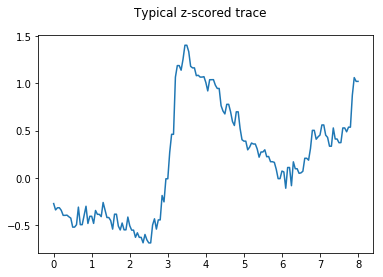
\includegraphics[width=\textwidth]{img/example_neuro_channel_zscored.png}
        \caption{Example Z-Scored Neuronal Trace}
        \label{fig:example_neuro_channel_zscored}
    \end{subfigure}\hspace{0.05\textwidth}
    %%
    \begin{subfigure}[b]{0.4\textwidth}
        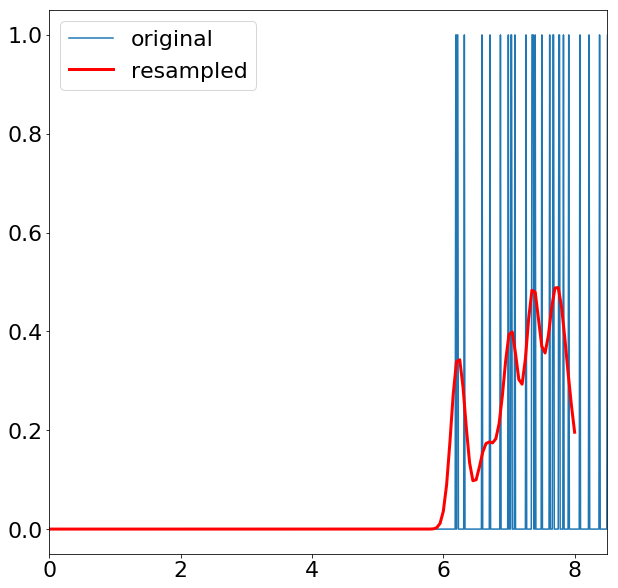
\includegraphics[width=\textwidth]{img/example_lick_rate_resampled.png}
        \caption{Example Lick Rate}
        \label{fig:example_lick_rate_resampled}
    \end{subfigure}
    %%
    \begin{subfigure}[b]{0.4\textwidth}
        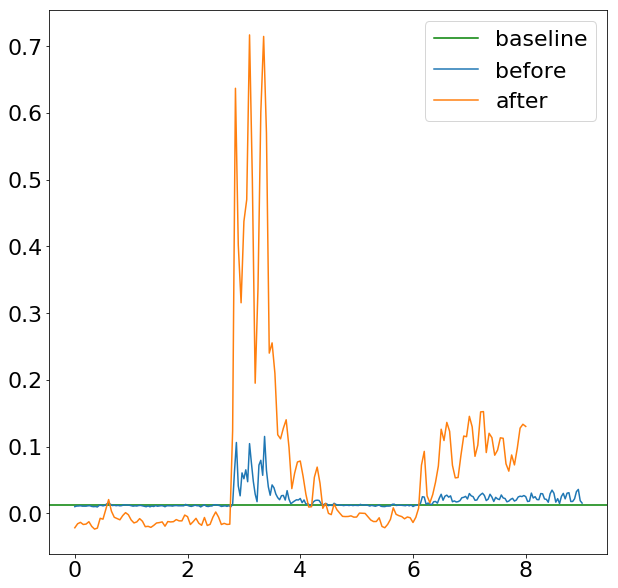
\includegraphics[width=\textwidth]{img/example_paw_move_resampled.png}
        \caption{Example paw movement amplitude}
        \label{fig:example_paw_move_resampled}
    \end{subfigure}\hspace{0.05\textwidth}
    %%
    \begin{subfigure}[b]{0.4\textwidth}
        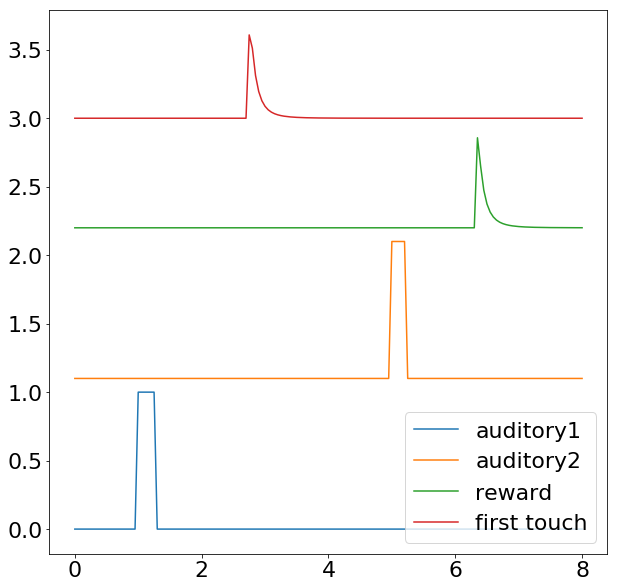
\includegraphics[width=\textwidth]{img/example_behav_signal.png}
        \caption{Other non-neuronal variables}
        \label{fig:example_behav_signal}
    \end{subfigure}
    \caption{Example behavioural and neuronal data during a typical 8 second trial (x-axis), resampled to neuronal sampling frequency of 20Hz and normalized across all trials}\label{fig:example_behavioural_neural_data}
\end{figure}

\section{Preliminary Exploratory Analysis}
We believe that it is advantageous to get familiar with the data using simple well-established metrics prior to using sophisticated model-based explanations, mainly to obtain intuition on whether the data is consistent with the assumptions of the models we later intend to fit. Firstly, we expect the measured neuronal signal to be autocorrelated, since the GCaMP6f timescale of ~500ms is larger than the sampling timestep of 50ms. Secondly, we expect the signals from different brain areas to be cross-correlated. Since the slowly-changing components of the signals can be linearised to a reasonable accuracy within the range of a few time steps, a zero cross-correlation would indicate that any coupling between channels is purely nonlinear and very weak compared to the signal magnitude.

As expected, the autocorrelation of the data resembles a decaying exponential function, indicating the presence of a slowly changing component [\cref{fig:example_neuro_autocorr}]. Further, the autocorrelation has an oscillatory component which is typical of a fastly changing signal convolved with a slowly decaying exponential. The cross-correlation of the data indicates clustering, as some channels are highly correlated to each other while not being correlated to other channels [\cref{fig:prelim_crosscorr_val,fig:prelim_crosscorr_del}]. In some cases, we observe a channel that is somewhat correlated to all other channels, while other channels are not correlated, indicating a propagation of some global brain state. Further, we decided to investigate how cross-correlation changes with learning. For this purpose, we define the synchronization coefficient as the average absolute value of the off-diagonal entries of the channel correlation matrix $C_{ij}$
\begin{equation}
  S = \frac{1}{N^2 - N}\sum_{ij} |C_{ij}| - \delta_{ij}
\end{equation}
and plot it as a function of the training day [\cref{fig:prelim_synchr}]. We see that the average synchronization between channels is 0.5, meaning that the data is highly correlated. Further, in several mice we observe a steep rise of synchronization to values of 0.8 or even 0.9 a few days after they have achieved expert level performance. This does not happen to all animals that reach expert level performance, so we are looking forwards to further investigate this observation in later works.

\begin{figure}
    \centering
    \begin{subfigure}[b]{0.4\textwidth}
        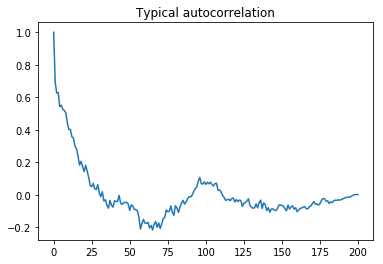
\includegraphics[width=\textwidth]{img/example_neuro_autocorr.png}
        \caption{Example value of autocorrelation of neuronal signal from a single channel}
        \label{fig:example_neuro_autocorr}
    \end{subfigure}\hspace{0.05\textwidth}
    %%
    \begin{subfigure}[b]{0.4\textwidth}
        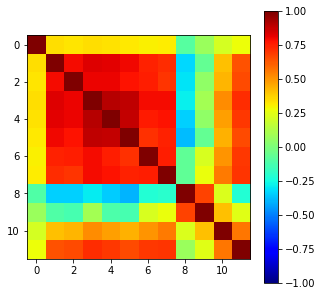
\includegraphics[width=\textwidth]{img/example_neuro_crosscorr_values.png}
        \caption{Example value of cross-correlation between channels of a 12 channel mouse}
        \label{fig:prelim_crosscorr_val}
    \end{subfigure}
    %%
    \begin{subfigure}[b]{0.4\textwidth}
        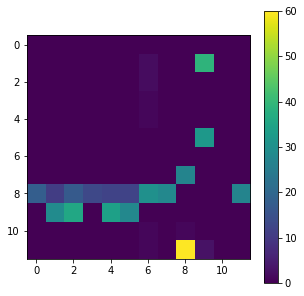
\includegraphics[width=\textwidth]{img/example_neuro_crosscorr_delays.png}
        \caption{Example delay of cross-correlation between channels of a 12 channel mouse}
        \label{fig:prelim_crosscorr_del}
    \end{subfigure}\hspace{0.05\textwidth}
    %%
    \begin{subfigure}[b]{0.4\textwidth}
        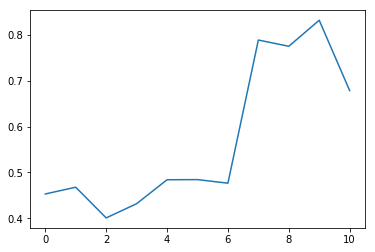
\includegraphics[width=\textwidth]{img/example_neuro_synchr_by_days.png}
        \caption{Example synchronization coefficient of the same mouse across days}
        \label{fig:prelim_synchr}
    \end{subfigure}
    \caption{Preliminary analysis of neuronal data}\label{fig:prelim_analysis_1}
\end{figure}



\section{MAR Model}
%We want to explore the capacity of existing models of mesoscopic neuronal dynamics to explain the collected data. Further, we want to compare the estimated functional connectivity and derived metrics, such as total number of links, their degree and clustering coefficient.

We have considered the following form of an autoregressive process
%%
\begin{equation}
  X_i(t) = \sum_{j=1}^p \sum_{k=1}^{N_X}   A^j_{ik} X_k(t-j) + \sum_{k=1}^{N_U} B_{ik} U_k(t-1) + \epsilon_i 
\end{equation}
where $X$ is the observed calcium signal, $U$ is the external input, $p$ is the maximal order of the MAR model, $A$ and $B$ are the unknown functional connectivity tensors. In this study we have investigated 3 different implementations of the above model: analytic unconstrained solution, numeric constrained and regularized solution and a bayesian model inversion framework by Penny et al \cite{penny_bayesian_2002}. In \cref{fig:features_mar_models} we present the comparison between features available in each implementation. Note that many of the features not present in the below table are reasonably easy to implement. We had to restrict ourselves only to the features that form the essential differences between the 3 implementations in order to be time-efficient. For the analytic and numeric model we derived and implemented an optimized solver for scratch. The reason not to use an existing library was the inability of libraries we found to handle fitting a MAR model to multiple trials simultaneously, which we believe is necessary to improve rigor of the estimated model parameters. The difference of the numerical model to the analytic was in additional $L_1$ regularization and a constraint requiring all $A$ matrix elements to be non-negative. We have chosen this constraint because all of the measured neuronal populations are excitatory. Most elements in an unconstrained estimated $A$ matrix are positive, and those that are negative are relativelty small, so we concluded that there is likely no real inhibitory effect between populations, and it makes sense to restrict it altogether. Finally, we have also used a Bayesian inversion-based MAR model implemented by Penny et el. \cite{penny_bayesian_2002} as part of the SPM toolbox. This model makes prior assumptions about the distributions of model parameters ($A$ matrix elements), their precisions, as well as the precisions of the added noise. Penny et al. \cite{penny_bayesian_2002} then proceed to invert the model using VB mean-field approximation, obtaining an iterative procedure for computing the model parameters and the associated model evidences.

\begin{table}[h!]
\centering
\begin{tabular}{l | l | l | l}
                            & Analytic & Numeric & Bayesian \\ \hline
  Arbitrary model order     & Yes & No & Yes \\ \hline
  External input            & Yes & No & No \\ \hline
  Optimization over trials  & Yes & Yes & No \\ \hline
  Non-negative constraint   & No  & Yes & No \\ \hline
  Regularization            & No  & Yes & Yes \\ \hline
  Model Selection Criteria  & AIC,BIC  & AIC,BIC & ME \\
\end{tabular}
\caption{Feature comparison between the 3 MAR models used}
\label{fig:features_mar_models}
\end{table}

We summarize the results of the above model estimates as follows
\begin{itemize}
 \item The $A$ matrix estimates for all model orders are diagonally-dominant, with $p=1$ being the most dominant order. This means that a large portion of a neuronal signal can be explained by its own past value. This is not surprising given the autocorrelation we have observed previously, and is expected of the slowly-decaying calcium indicator signals.
 \item The $A$ matrix estimates experience small changes in presence of the external observables $U$, but qualitatively they stay diagonally-dominant [\cref{fig:marN_analytic_noinput_A1,fig:marN_analytic_withinput_A1}].
 \item Similarly, the $A$ matrix estimate appears qualitatively the same when computed separately for each performance class (Go, Nogo, Miss, False Alarm) [\cref{fig:marN_analytic_withinput_A1_ByPerformance}]
 \item The $A$ matrix estimates based on Bayesian inversion appear to have stronger off-diagonal entries than the other methods [\cref{fig:marN_penny_noinput_A1_avg}]. It is hard to judge whether this estimate is more accurate than that of the analytic models. On one hand, the Bayesian model starts with the diagonal prior for the $A$ matrix, so having more off-diagonal entries in not the result of a local minima. From the other, it has more rigorous estimation of the noise covariance which would in principle make it more accurate. However, unlike our analytic estimate, it has a downside of not being able to combine all trials into one estimate, which dramatically reduces the amount of data points available to the method compared to the analytic one, potentially resulting in spurious connections due to noise fitting.
 \item The $A$ matrix estimates based on numeric regularized approach demonstrate comparable model fitness while having most entries set to zero [\cref{fig:mar1_numeric_constr_A1}]. Interestingly, many diagonal entries are zero, suggesting that the signal of the associated channels can be to some extent explained by other channels. In particular, it is clearly visible that channel 3 correlates with all other channels, indicating some sort of whole-brain activity.
 \item Input matrix $U$ appears quite informative [\cref{fig:marN_analytic_withinput_B1}]. For example, paw movement appears to be positively correlated with most of the channels, while reward is correlated with channels 5 and 7.
 \item For the analytic models, the loss function improves roughly by 2\% per order up to order 3, then by 1\% up to order 7. AIC and BIC are not significant compared to the original loss function for orders up to 10 [\cref{fig:MAR_AIC_BIC}]. On the contrary, the model evidence, as estimated by the Penny \cite{penny_bayesian_2002} model, appears to go down dramatically with increasing model order, suggesting log bayesian group factors of the order of -20 for each following model order [\cref{fig:marN-penny-model-evidence}]. It is likely that at least one of the model selection criteria we have used has a bug, but we are not able to resolve it at this time.
\end{itemize}


\begin{figure}
    \centering
    \begin{subfigure}[b]{0.4\textwidth}
        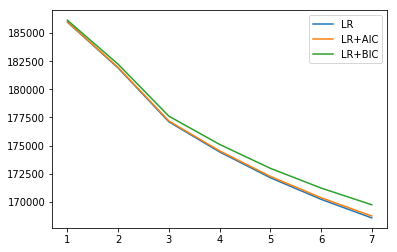
\includegraphics[width=\textwidth]{img/marN_analytic_noinput_aicbic.png}
        \caption{MAR without input}
        \label{fig:marN_analytic_noinput_aicbic}
    \end{subfigure}\hspace{0.05\textwidth}
    %%
    \begin{subfigure}[b]{0.4\textwidth}
        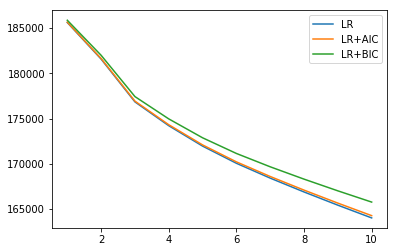
\includegraphics[width=\textwidth]{img/marN_analytic_withinput_aicbic.png}
        \caption{MAR with input}
        \label{fig:marN_analytic_withinput_aicbic}
    \end{subfigure}\hspace{0.03\textwidth}
    \caption{Akaike and Bayesian Information Criteria for MAR model fit as a function of model order.}
    \label{fig:MAR_AIC_BIC}
\end{figure}

\begin{figure}
  \centering
  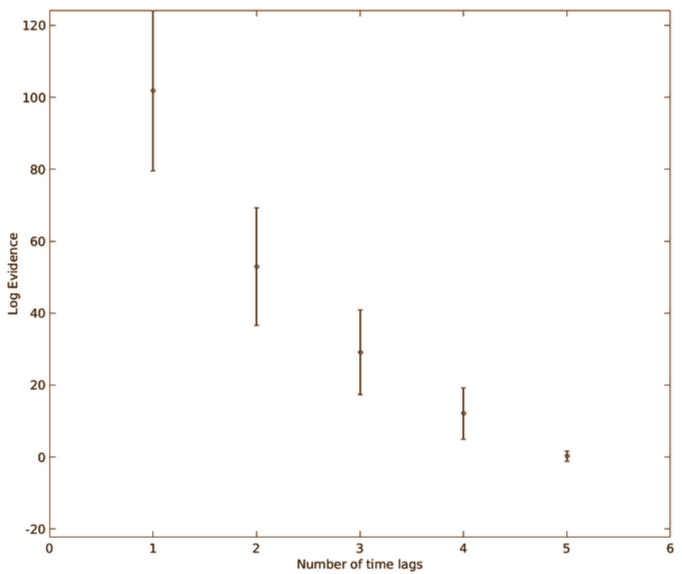
\includegraphics[width=0.5\textwidth]{img/marN-penny-model-evidence.png}
  \caption{Mean and variance of inter-trial log Model Evidence for MAR model as a function of model order}
  \label{fig:marN-penny-model-evidence}
\end{figure}


\begin{figure}
    \centering
    \begin{subfigure}[b]{0.4\textwidth}
        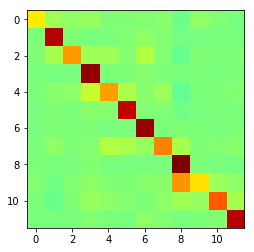
\includegraphics[width=\textwidth]{img/marN_analytic_noinput_A1.png}
        \caption{Analytic Estimate Without Input}
        \label{fig:marN_analytic_noinput_A1}
    \end{subfigure}\hspace{0.05\textwidth}
    %%
    \begin{subfigure}[b]{0.4\textwidth}
        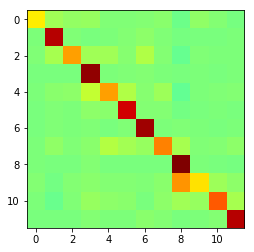
\includegraphics[width=\textwidth]{img/marN_analytic_withinput_A1.png}
        \caption{Analytic Estimate With Input}
        \label{fig:marN_analytic_withinput_A1}
    \end{subfigure}
    %%
    \begin{subfigure}[b]{0.4\textwidth}
        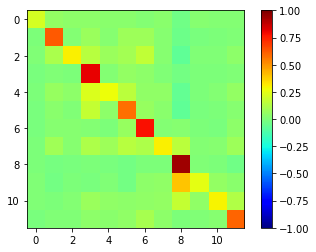
\includegraphics[width=\textwidth]{img/marN_penny_noinput_A1_avg.png}
        \caption{Bayesian Inversion Estimate Without Input}
        \label{fig:marN_penny_noinput_A1_avg}
    \end{subfigure}\hspace{0.05\textwidth}
    %%
    \begin{subfigure}[b]{0.4\textwidth}
        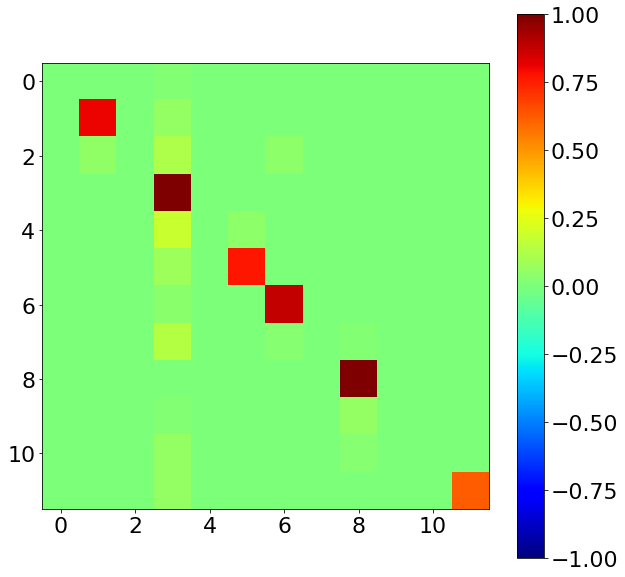
\includegraphics[width=\textwidth]{img/mar1_numeric_constr_A1.png}
        \caption{Numeric Regularized Estimate Without Input}
        \label{fig:mar1_numeric_constr_A1}
    \end{subfigure}
    \caption{MAR $A_1$ matrices estimated using different approaches to model fitting}\label{fig:marN_A1_estimate_by_method}
\end{figure}

\begin{figure}
  \centering
  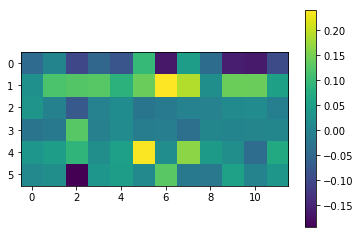
\includegraphics[width=0.5\textwidth]{img/marN_analytic_withinput_B1.png}
  \caption{Analytic Estimate Of Input Matrix. Horizontal axis denotes neuronal channels, vertical denotes input variables. In order, the input variables are: lick rate, paw movement, starting auditory cue, report auditory cue, reward and first touch}
  \label{fig:marN_analytic_withinput_B1}
\end{figure}







\begin{figure}
    \centering
    \begin{subfigure}[b]{0.4\textwidth}
        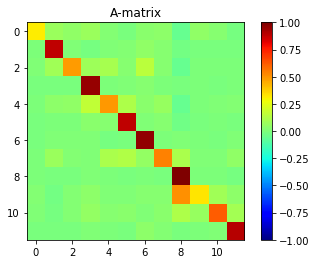
\includegraphics[width=\textwidth]{img/marN_analytic_withinput_A1_Go.png}
        \caption{Go}
        \label{fig:marN_analytic_withinput_A1_Go}
    \end{subfigure}\hspace{0.05\textwidth}
    %%
    \begin{subfigure}[b]{0.4\textwidth}
        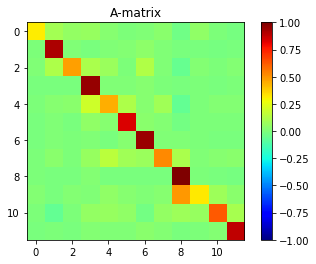
\includegraphics[width=\textwidth]{img/marN_analytic_withinput_A1_Nogo.png}
        \caption{NoGo}
        \label{fig:marN_analytic_withinput_A1_Nogo}
    \end{subfigure}
    %%
    \begin{subfigure}[b]{0.4\textwidth}
        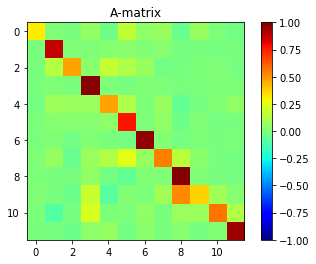
\includegraphics[width=\textwidth]{img/marN_analytic_withinput_A1_Miss.png}
        \caption{Miss}
        \label{fig:marN_analytic_withinput_A1_Miss}
    \end{subfigure}\hspace{0.05\textwidth}
    %%
    \begin{subfigure}[b]{0.4\textwidth}
        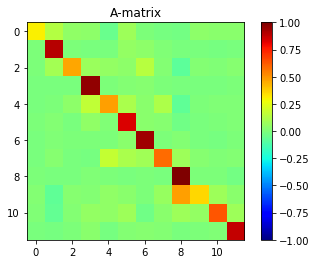
\includegraphics[width=\textwidth]{img/marN_analytic_withinput_A1_FA.png}
        \caption{False Alarm}
        \label{fig:marN_analytic_withinput_A1_FA}
    \end{subfigure}
    \caption{MAR $A_1$ matrix estimates for different performance classes}
    \label{fig:marN_analytic_withinput_A1_ByPerformance}
\end{figure}




\subsection{Linear Classifiability}

In this section, we decided to test if the neuronal signals were predictive of mouse performance. For simplicity, we restricted the predictive capacity of the data to that of a linear classifier trained on it. A simple way to test if data is predictive of the associated labels is to set the null hypothesis "It is not possible to predict the labels from the data better than chance", and then test for the level of confidence at which the null hypothesis can be rejected. Firstly, in order to avoid fitting the noise, we performed dimensionality reduction on the data using PCA, and selected only PC's with eigenvalues greater than $10^{-2}$ [\cref{fig:neuro_pca_eval}]. Then, we trained a binary linear classfier for each of the 4 possible performance outcomes in order to obtain classification accuracy of the true labels. Finally, we permuted the labels multiple times, re-training the classifiers every time. This approach worked nicely for GO and NOGO trials [\cref{fig:neuro_classifiability_go,fig:neuro_classifiability_nogo}]. The number MISS and FA trials form only a very small proportion of the whole trial set, which resulted in high classification accuracies happening by chance. In order to obtain a more rigorous estimate, we proceeded to randomly select a subset of non-MISS trials of number equal to that of the MISS trials, estimate the true and permuted classification accuracies, then repeat the whole process 10000 times. We can conclude that it is possible to construct a classifier identifying GO and NOGO trials from neuronal data with accuracy of the order of 90\%, rejecting the null hypothesis with z-scores of the order of 20. For FA it is possible to demonstrate rejection of the null hypothesis with z-score of 3.8, for MISS it is negligible. We conclude that more data is required to make robust statements about accuracy of linear classifiability for MISS and FA trials.

A question more important to this study is whether the performance classes can be predicted from the estimated FC, as that might indicate the use of different neuronal pathways during different behaviour. Inspecting the bulk-trial estimates of $A_1$ matrices for each performance class by eye, we were able to tell apart small differences, but fundamentally they appeared quite similar [\cref{fig:marN_analytic_withinput_A1_ByPerformance}]. To clarify this question, we repeated the same procedure as for the neuronal signals: dimensionality reduction [\cref{fig:marN_penny_pca_eval}], followed by true and shuffled linear classification accuracy estimation [\cref{fig:marN_penny_noinput_A1_classifiability}]. The results are essentially the same as for the neuronal signals. It is very much possible to classify GO and NOGO trials, albeit now the classfication accuracy is 88\% and 82\% and the z-scores are 14.5 and 9.5 respectively. Our conclusion about the classifiability of MISS and FA trials is the same as for the previous scenario.


\begin{figure}
  \centering
  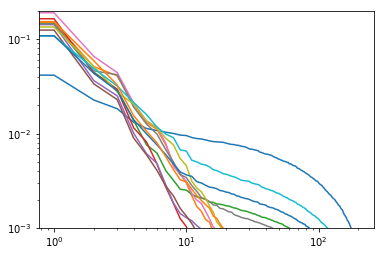
\includegraphics[width=0.5\textwidth]{img/example_neuro_PCA_eval_bychannel.png}
  \caption{Eigenvalue magnitude of neuronal signals of 12 channel mouse. Color denotes individual channels}
  \label{fig:neuro_pca_eval}
\end{figure}

\begin{figure}
  \centering
  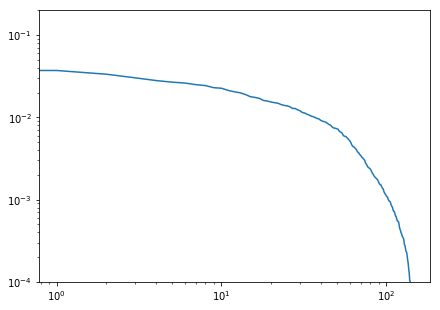
\includegraphics[width=0.5\textwidth]{img/marN_penny_noinput_A1_PCA_eval.png}
  \caption{Eigenvalue magnitude of MAR $A_1$ matrix}
  \label{fig:marN_penny_pca_eval}
\end{figure}



\begin{figure}
    \centering
    \begin{subfigure}[b]{0.4\textwidth}
        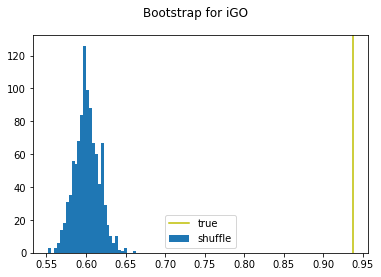
\includegraphics[width=\textwidth]{img/example_neuro_classifiability_go.png}
        \caption{Go. Z-score 21.5}
        \label{fig:neuro_classifiability_go}
    \end{subfigure}\hspace{0.05\textwidth}
    %%
    \begin{subfigure}[b]{0.4\textwidth}
        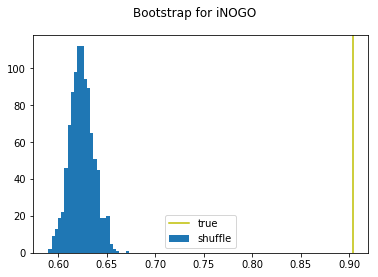
\includegraphics[width=\textwidth]{img/example_neuro_classifiability_nogo.png}
        \caption{NoGo. Z-score 22.3}
        \label{fig:neuro_classifiability_nogo}
    \end{subfigure}
    %%
    \begin{subfigure}[b]{0.4\textwidth}
        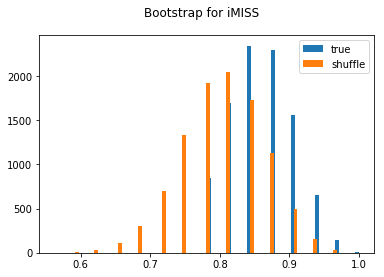
\includegraphics[width=\textwidth]{img/example_neuro_classifiability_miss.png}
        \caption{Miss. Z-score 0.62}
        \label{fig:neuro_classifiability_miss}
    \end{subfigure}\hspace{0.05\textwidth}
    %%
    \begin{subfigure}[b]{0.4\textwidth}
        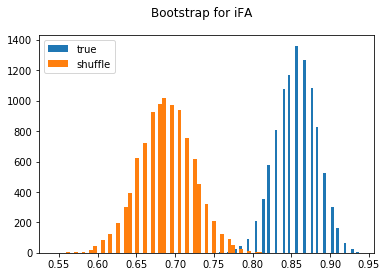
\includegraphics[width=\textwidth]{img/example_neuro_classifiability_fa.png}
        \caption{False Alarm. Z-score 3.8}
        \label{fig:neuro_classifiability_fa}
    \end{subfigure}
    \caption{Classifiability of mouse performance from neuronal data}\label{fig:neuro_classifiability}
\end{figure}


\begin{figure}
    \centering
    \begin{subfigure}[b]{0.4\textwidth}
        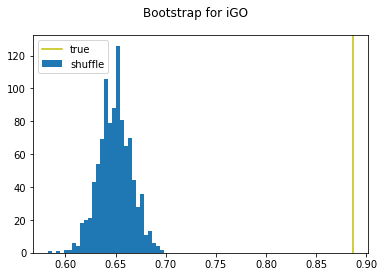
\includegraphics[width=\textwidth]{img/marN_penny_noinput_A1_classifiability_go.png}
        \caption{Go. Z-score 14.5}
        \label{fig:marN_penny_noinput_A1_classifiability_go}
    \end{subfigure}\hspace{0.05\textwidth}
    %%
    \begin{subfigure}[b]{0.4\textwidth}
        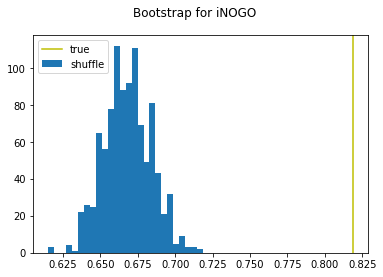
\includegraphics[width=\textwidth]{img/marN_penny_noinput_A1_classifiability_nogo.png}
        \caption{NoGo. Z-score 9.57}
        \label{fig:marN_penny_noinput_A1_classifiability_nogo}
    \end{subfigure}
    %%
    \begin{subfigure}[b]{0.4\textwidth}
        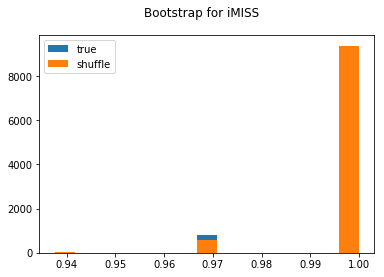
\includegraphics[width=\textwidth]{img/marN_penny_noinput_A1_classifiability_miss.png}
        \caption{Miss. Z-score -0.05}
        \label{fig:marN_penny_noinput_A1_classifiability_miss}
    \end{subfigure}\hspace{0.05\textwidth}
    %%
    \begin{subfigure}[b]{0.4\textwidth}
        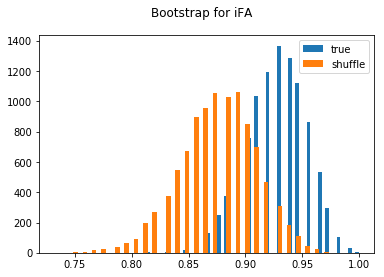
\includegraphics[width=\textwidth]{img/marN_penny_noinput_A1_classifiability_fa.png}
        \caption{False Alarm. Z-score 1.18}
        \label{fig:marN_penny_noinput_A1_classifiability_fa}
    \end{subfigure}
    \caption{Classifiability of mouse performance from MAR-estimated functional connectivity}\label{fig:marN_penny_noinput_A1_classifiability}
\end{figure}


\section{DCM Model}
While I have not found sufficient time to complete this analysis within the given time frame, it is intended to do this analysis for the following publication. For this purpose, I outline the steps necessary for the analysis. In a recent paper \cite{jung_dynamic_2019} Jung et al. have proposed a DCM paradigm to model calcium imaging data. We intend to use their result as a starting point.

\subsection{Latent variable model}
DCM models make use of two sets of equations - the latent variable equation, which self-consistently models the dynamics of latent variables and external inputs, as well as the forwards model, which computes the observable values based on the latent variables. Typically, DCM models make use of the neuronal state equation \cite{stephan_dynamic_2007}
%%
\begin{equation}
   \vec{x}(t+1) = A\vec{x}(t) + B \vec{x}(t) \vec{u}(t) + C\vec{u}(t) + \nu, \;\;\;\;\; \nu \sim \mathcal{N}(\vec{\mu}, \Sigma)
\end{equation}
%%
Instead \cite{jung_dynamic_2019} follow the convolution-based model based on the work of Moran et al \cite{moran_neural_2013} . The membrane potential of a neuronal population is given by a convolution of a non-linear function of internal and external input with a suitable kernel
%%
\begin{equation}
   V_i(t) = h_{i}(t) \otimes (Inp_i(t) + \Sigma_j \gamma_{ij} \sigma_j(V_i - T_i))
\end{equation}
%%  
where $i$ denotes the index of a neuronal population, $Inp_i(t)$ is the external input to each neuron, $\gamma_{ij}$ are the connection weights,  is the nonlinear activation function, $T_i$ is the firing threshold, the non-linear transfer function is given by
%%
\begin{equation}
   \sigma_i(V_i - T_i) = \frac{f_{max}}{1 - e^{R(V_i - T_i)}}
\end{equation}
%%
and the kernel is given by
%%
\begin{equation}
   h_i(t) = H_i k_i t e^{-k_i t}
\end{equation}
%%
Using differentiation, the above equation can be rewritten in the form of an ODE
%%
\begin{eqnarray}
\dot{V}_i &=& I_i \\
\dot{I}_i &=& k_i H_i (Inp_i + \Sigma_j \gamma_{ij} \sigma_j(V_i - T_i))) - 2k_i \dot{V}_i - k_i^2 (V_i - T_i)
\end{eqnarray}
%%
where $I$ is the membrane current. This model is effectively a set of damped harmonic oscillators, coupled together by a nonlinear transfer function.

\subsection{Forwards model}
Jung et al. \cite{jung_dynamic_2019} use the forwards model designed by Rahmati et al\cite{rahmati_inferring_2016} to estimate the calcium signal from the membrane potential.
%%
\begin{equation}
   \frac{d}{dt}[Ca^{2+}] = K_{ca} g_{ca} \sigma(V_i - T_i) - \frac{[Ca^{2+}] - [Ca^{2+}]_{base}}{\tau_{ca}}
\end{equation}
\begin{equation}
   F = d_F + k_F \frac{[Ca^{2+}]}{[Ca^{2+}] + k_d}
\end{equation}
%%
Thus, in the absence of noise, the variables $V(t), I(t)$ and $[Ca^{2+}](t)$ form a deterministic dynamical system, enabling us to compute their values any time in the future given suitable initial conditions.

\subsection{Observer noise}

The simplest problem in DCM is model inversion under observer noise. Namely, the measured fluorescence is assumed to be sampled from a multivariate normal distribution with some (generally unknown) covariance matrix. The mean of the distribution is then given by the forwards model
%%
\begin{equation}
   F_m(t) \sim \mathcal{N}(F(t), \Sigma)
\end{equation}
%%
In this case, the likelihood function $P[F_m(t) | \theta(t)]$ is given by
%%
\begin{equation}
   P[F_m(t) | \theta(t)] = Gau(F_m(t) - F(t, \theta(t)), \Sigma)
\end{equation}
%%
And the total likelihood of the data.
%%
\begin{equation}
   L[F_m | \theta] = \prod_t Gau(F_m(t) - F(t, \theta(t)), \Sigma)
\end{equation}
%%
The unknown parameters at time $t$ are given by the time-changing latent variables, as well as some unknown constants of the model
%%
\begin{equation}
   \theta(t) = \{V(t), I(t), [Ca^{2+}](t), \gamma_{ij}, \tau, ...\}
\end{equation}
%%
Now, since the $\theta(t)$ are not known, it would make sense to eliminate them from the model. Using the fact that the model is deterministic, we can replace $F$ with an equivalent function $\tilde{F}$, which only requires initial values of parameters to compute the estimate of the observed signal
\begin{equation}
   F(t, \theta(t) = \tilde{F}(t, \theta(0))
\end{equation}
$\tilde{F}$ is can be computed using the following algorithm
\begin{itemize}
  \item Initialize the latent variable ODE at time $t=0$ using provided values of $\theta(0)$
  \item Forwards-integrate ODE to get values of $\theta(t_i)$ for desired time points $\{t_i\}$
  \item Evaluate $\tilde{F} = F(t_i, \theta(t_i))$ using the forwards model 
\end{itemize}

\subsection{Model Inversion}

This is how far we got with the model at the moment. While Jung et al. \cite{jung_dynamic_2019} claim to have used SPM for their analysis, no details of the procedure of model inversion is given in their publication. It is fairly clear that given the complexity of the likelihood function, approximations such as Laplace or mean-field are not not computable analytically. Therefore, a numerical MCMC-like computation of optimal parameters and model evidence appears to be the only feasible solution. However, a brief look at the SPM toolbox seems to suggest that other DCM models implemented in it are using VB approach, although more effort is necessary to understand how exactly it is implemented. Perhaps there exists a numerical method to approximate mean-field integrals from VB approach?

\section{Acronyms}

\begin{tabular}{l l}
        AIC     &       Akaike Information Criterion \\
        BIC     &       Bayesian Information Criterion \\
	DCM	&	Dynamical Causal Model\\
	EEG	&	Electroencephalography\\
	FC	&	Functional Connectivity\\
	fMRI	&	Functional Magnetic Resonance Imaging\\
	KL	&	Kullbeck-Liebler (Divergence)\\
	MAR	&	Multivariate Autoregressive (Model)\\
	MCMC &  Markov Chain Monte Carlo\\
	MI	&	Mutual Information\\
	ME	&	Model Evidence\\
	TE	&	Transfer Entropy\\
	VB  &   Variational Bayes
\end{tabular}

\printbibliography

\end{document}
